\section{Experiments}

\subsection{Design of N-tuple Networks and Vertical Split Encoding for 2048}

6, 7, 8, 9 タプルをデザインした.デザインにあたっては,「妥当そうに見える形を平行移動する」方策を用いた.
6タプルでは,4つの形を選定し,それらを平行移動してできる9つの組合せとした.
7タプルでは,4つの形を選定し,それらを平行移動してできる8つの組合せとした.
8タプルでは,3つの形を選定し,それらを平行移動してできる5つの組合せとした.
6タプルでは,4つの形を選定し,それらを平行移動してできる7つの組合せとした.

それぞれの N-Tuple について,各パラメータを 64 bits,後述する TC 学習を用いて64 GBメモリに収まることを要件として,VSE の value ranges を設計した.
6タプルの場合は VSE なしで十分メモリに収まる.
7タプルの場合には,少なくとも 2 つに分ける必要があり,2つのvalue ranges の大きさが 11 + 10 となるように分けた.
8タプルの場合には,少なくとも 3 つに分ける必要があり,3つのvalue ranges の大きさが 9 + 9 + 6 となるように分けた.
9タプルの場合には,少なくとも 4 つに分ける必要があり,4つのvalue ranges の大きさが 7 + 7 + 7 + 6 となるように分けた.

各タプルについて,Multistaging としてゲームの進行に応じて、重みを参照するテーブルを切り替える手法である。本研究では 2 ステージとし、タイル 32768 が生成される前後でネットワークを切り替えるように設計した。

VSE の value ranges の取り方はもう少し自由度がある.それらを網羅的に試すのは今後の課題である.

\subsection{Training and Evaluation with Expectimax Search}

上のように定義した N-tuple networks に対し,強化学習によってパラメータを調整した.
学習には,Temporal Coherence 学習を用いた.
	Temporal coherence 学習(TC 学習)
学習率を自動的に調整する機能を備えた TD 学習であり、Jaśkowski によって初めて 2048 に導入された手法である。本研究における N タプルネットワークの学習では、効率的かつ安定的な収束のために TC 学習を採用した。
	Optimistic initialization(OI)
学習初期段階での探索を広く行うために、重みをゼロではなく大きな値で初期化する手法である。本研究では、すべての afterstate の初期値が 320,000 となるように重みを初期化した。
OI 以外には,Exploration は入れていない.局所最適にならないよう,TC 学習で学習率を決定するパラメータを初期化する.step ごと.

本研究では実験として6,7,8,9のそれぞれのタプルと既存研究で用いたタプルの5種類についてそれぞれ2.0e11 step分学習を行い,1e9 ごとにパラメータを出力しGreedyプレイとExpectimaxプレイでそれぞれ評価を行った.
なお,random 要素の対応として,5つの異なるseedを用いて学習を行った.

図 \ref{fig:exp2} にtraining curve を示す.

\begin{figure}
 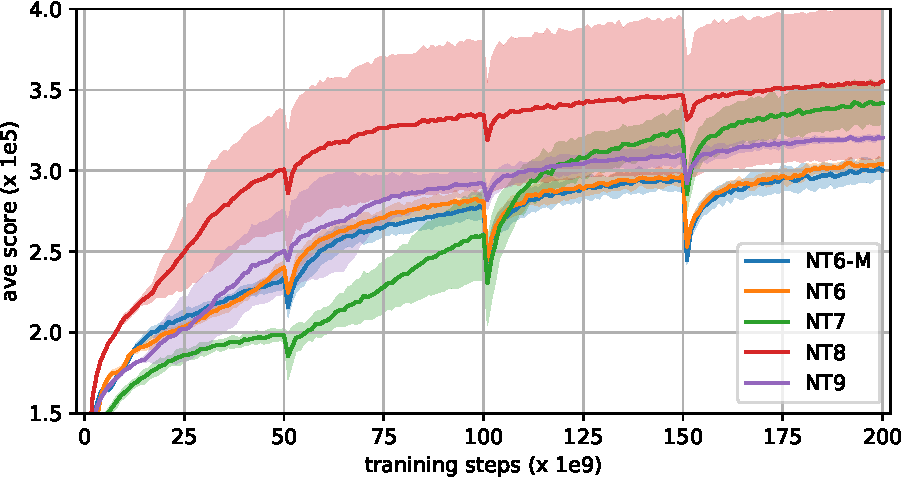
\includegraphics[width=.95\linewidth]{figures/plot-exp2.pdf}
 \caption{Training curve (evaluated with 10000 games of the greedy play)}
 \label{fig:exp2}
\end{figure}

グラフから分かること.


最終的に得られたN-tuple network を用いて,Expectimax 探索 (3-ply, 5-ply) と組合せた評価も行った.
結果を \ref{table:exp3} に示す.

表から分かること.

\begin{table}
 \caption{Experiment results}
 \label{table:exp3}
 \small\begin{tabular}{l|l|l|l|l|l|l|l|l|l}
  \hline \hline
  & \multicolumn{2}{c}{1-ply (10000 games)} & \multicolumn{2}{c}{3-ply (1000 games)} & \multicolumn{2}{c}{5-ply (100 games)} \\
  & ave. score & 32768[\%] & ave. score & 32768[\%] & ave. score & 32768[\%] \\
  \hline
   NT0 (no VSE) & 300241$\pm$\phantom{0}5922	& 14.3$\pm$\phantom{0}1.7		& 462677$\pm$15573		& 44.3$\pm$\phantom{0}4.7		& 508618$\pm$\phantom{0}15010	& 55.0$\pm$\phantom{0}4.9 \\ \hline
   NT6 (no VSE) & 304149$\pm$\phantom{0}4361	& 14.9$\pm$\phantom{0}0.4		& 481544$\pm$\phantom{0}5497	& 47.8$\pm$\phantom{0}0.4	& 533801$\pm$\phantom{0}18084	& 61.3$\pm$\phantom{0}5.0 \\ \hline
   NT7 (2-VSE)	& 342009$\pm$12427		& 19.1$\pm$\phantom{0}2.9		& 491425$\pm$19140		& 46.1$\pm$\phantom{0}5.1		& 550848$\pm$\phantom{0}19390	& 60.5$\pm$\phantom{0}5.1 \\\hline
   NT8 (3-VSE)	& 355420$\pm$47102		& 15.5$\pm$15.6				& 438702$\pm$91280		& 29.1$\pm$29.1		& 448579$\pm$102127	& 31.5$\pm$32.0 \\\hline
   NT9 (4-VSE)	& 320205$\pm$\phantom{0}1404	& \phantom{0}0.0$\pm$\phantom{0}0.0	& 360286$\pm$\phantom{0}1446	& \phantom{0}0.0$\pm$\phantom{0}0.0		& 363160$\pm$\phantom{00}1886	& \phantom{0}0.0$\pm$\phantom{0}0.0 \\\hline
 \end{tabular}
\end{table}

\subsection{Evaluation of Best N-tuple Networks}

特に,NT8 で学習がうまくいったものとうまくいかなかったものがあったので,9タプルを除くそれぞれのNTupleの大きさについて,
5つの学習のうちもっともうまくいったネットワークを用いての評価を行った.
1つのネットワークに対して,5つの異なるシードでテストプレイ (1-ply, 3-ply, 5-ply) を行った結果を表 \ref{table:exp4} に示す.

表から分かること.


\begin{table}
 \caption{Results of best agents}
 \label{table:exp4}
 \small\begin{tabular}{l|l|l|l|l|l|l|l|l|l}
  \hline \hline
  & \multicolumn{2}{c}{1-ply (10000 games)} & \multicolumn{2}{c}{3-ply (1000 games)} & \multicolumn{2}{c}{5-ply (100 games)} \\
  & ave. score & 32768[\%] & ave. score & 32768[\%] & ave. score & 32768[\%] \\
  \hline
   best NT0 (no VSE)	& 311\,354$\pm$1\,971		& 16.9$\pm$0.3	& 484\,281$\pm$5\,435	& 49.0$\pm$1.2	& 517\,595$\pm$17\,160	& 56.2$\pm$5.7 \\\hline
   best NT6 (no VSE)	& 300\,410$\pm$1\,122		& 14.4$\pm$0.4	& 484\,718$\pm$6\,182	& 48.1$\pm$1.0	& 532\,599$\pm$28\,947	& 58.4$\pm$8.5 \\\hline
   best NT7 (2-VSE)	& 341\,636$\pm$1\,719		& 19.0$\pm$0.2	& 484\,328$\pm$6\,187	& 44.2$\pm$1.9	& 541\,210$\pm$22\,938	& 56.6$\pm$5.8 \\\hline
   best NT8 (3-VSE)	& 407\,206$\pm$\phantom{1\,}432 & 30.0$\pm$0.2	& 547\,365$\pm$4\,938	& 57.2$\pm$1.9	& 587\,690$\pm$20\,439	& 66.2$\pm$6.2 \\\hline
 \end{tabular}
\end{table}
